%\renewcommand{\thechapter}{Related work} 
%\renewcommand{\chaptername}{Related work} % To supress the Chaper from appearing 
\chapter{Related work} 

\ifpdf
    \graphicspath{{Chapter1/Chapter1Figs/PNG/}{Chapter1/Chapter1Figs/PDF/}{Chapter1/Chapter1Figs/}}
\else
    \graphicspath{{Chapter1/Chapter1Figs/EPS/}{Chapter1/Chapter1Figs/}}
\fi
\doublespacing
HPC systems depend on hardware and software to function appropriately. 

\section{Section title}
\label{sec:2.1}
... Place your section contents ....
\subsection{first subsection}
... and some more 

\section{Section title}
\label{sec:2.2}
... Place your section contents ....
\subsection{Second subsection }
... and some more 

\section{Section title}
\label{sec:2.3}
... Place your section contents ....

\section{Section title}
\label{sec:2.4}
... Place your section contents ....

\section{Section title}
\label{sec:2.5}
... Place your section contents ....

\begin{figure}[H]
\large
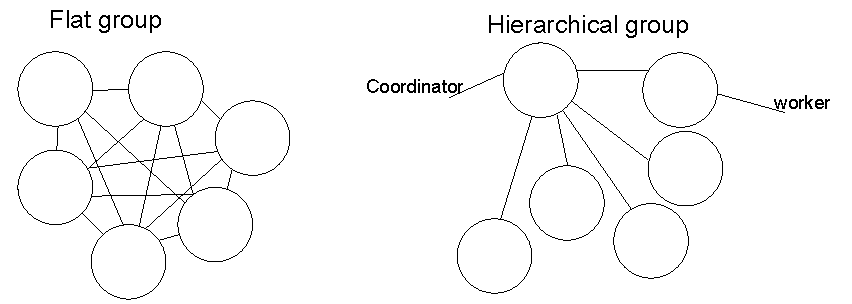
\includegraphics[width=16cm, height=7cm]{fault_masking.pdf}
\vspace{-0.5cm}\caption{Flat group and hierarchical group masking}
\label{fig:4}
%\label{fig:flate}
\end{figure}

%I would also like to add an extra bookmark in acroread like so ...
\ifpdf
  \pdfbookmark[2]{bookmark text is here}{And this is what I want bookmarked}
\fi
% ------------------------------------------------------------------------


%%% Local Variables: 
%%% mode: latex
%%% TeX-master: "../thesis"
%%% End: 
